%Correct the file name.
%X: book number
%Y: part number
%ZZZ: page number in three digits. So page 3 would be 003.

\documentclass[11pt]{amsbook}

\usepackage{../HBSuerDemir}	% ------------------------


\begin{document}

hypothesis of (1) is satisfied when we replace $a$ by $a^{-1}$ and $b$ by $b^{-1}$. Using (1) with $a^{-1} , b^{-1}$ in place
of $a,b$, respectively, we obtain \[(ab)^{-n} = ((ab)^{-1})^n = (a^{-1} b^{-1})^n = (a^{-1})^n (b^{-1})^n = a^{-n} b^{-n} \]
for $n \in \mathbb{N} $. Thus $(ab)^n = a^n b^n$ is valid also when $n \leq -1$. So $(ab)^n = a^n b^n$ for all $n\in \mathbb{Z}$.

\begin{lem}
Let $G$ be a commutative group. Then $(ab)^n = a^n b^n$ for all $a,b\in G $ and for all $n\in \mathbb{Z}$
\end{lem}

\begin{proof}
This follows immediately from Lemma 8.14.
\end{proof}
So far, we dealt with multiplicative groups. For additive groups, there
are some modifications. In the case of an  additive group, the unique element in $P_n (a_1 , a_2 ,..., a_n)$
of Lemma 8.3 is called the sum of $a_1 , a_2 ,..., a_n$ and is denoted by $a_1 + a_2 +....+ a_n$ or by $\sum_{i=1}^n a_i$.
We write $na$ for $a_1 + a_2 +....+ a_n$ in case $n\in \mathbb{N}$ and $a_1 , a_2 ,..., a_n$ are all equal to $a\in G$. Also, 
we define $0a=0$(the first 0 is the integer 0, the second 0 is the identity element of $G$) and $(-m)a = -(ma)$
for $m\in \mathbb{N}$. Thus we defined $na$ for all $n\in \mathbb{Z} , a\in G $.

\begin{lem}
Let G be a additively written commutative group. Then
\begin{enumerate}
	\item $ma+na=(m+n)a$
	\item $(-m)a = m(-a)$
	\item $n(ma)=(nm)a$
	\item $n(a+b)=na+nb$
\end{enumerate}
for all $m,n\in \mathbb{Z} ,a,b\in G$
\end{lem}

\begin{proof}
(1),(2),(3) foolow from Lemma 8.7 and (4) from Lemma 8.15.
\end{proof}

Notice that commutativity is essential for (4).
\par

\begin{center}
Exercises
\end{center}

\begin{enumerate}
\item Let G be a group such that $a^2=1$ for all $a\in G$. Prove that G is commutative.
\end{enumerate}



% =======================================================
\end{document}  

%==== templates ====

%==== environments ====

%\begin{figure}[htb]
%	\centering
%	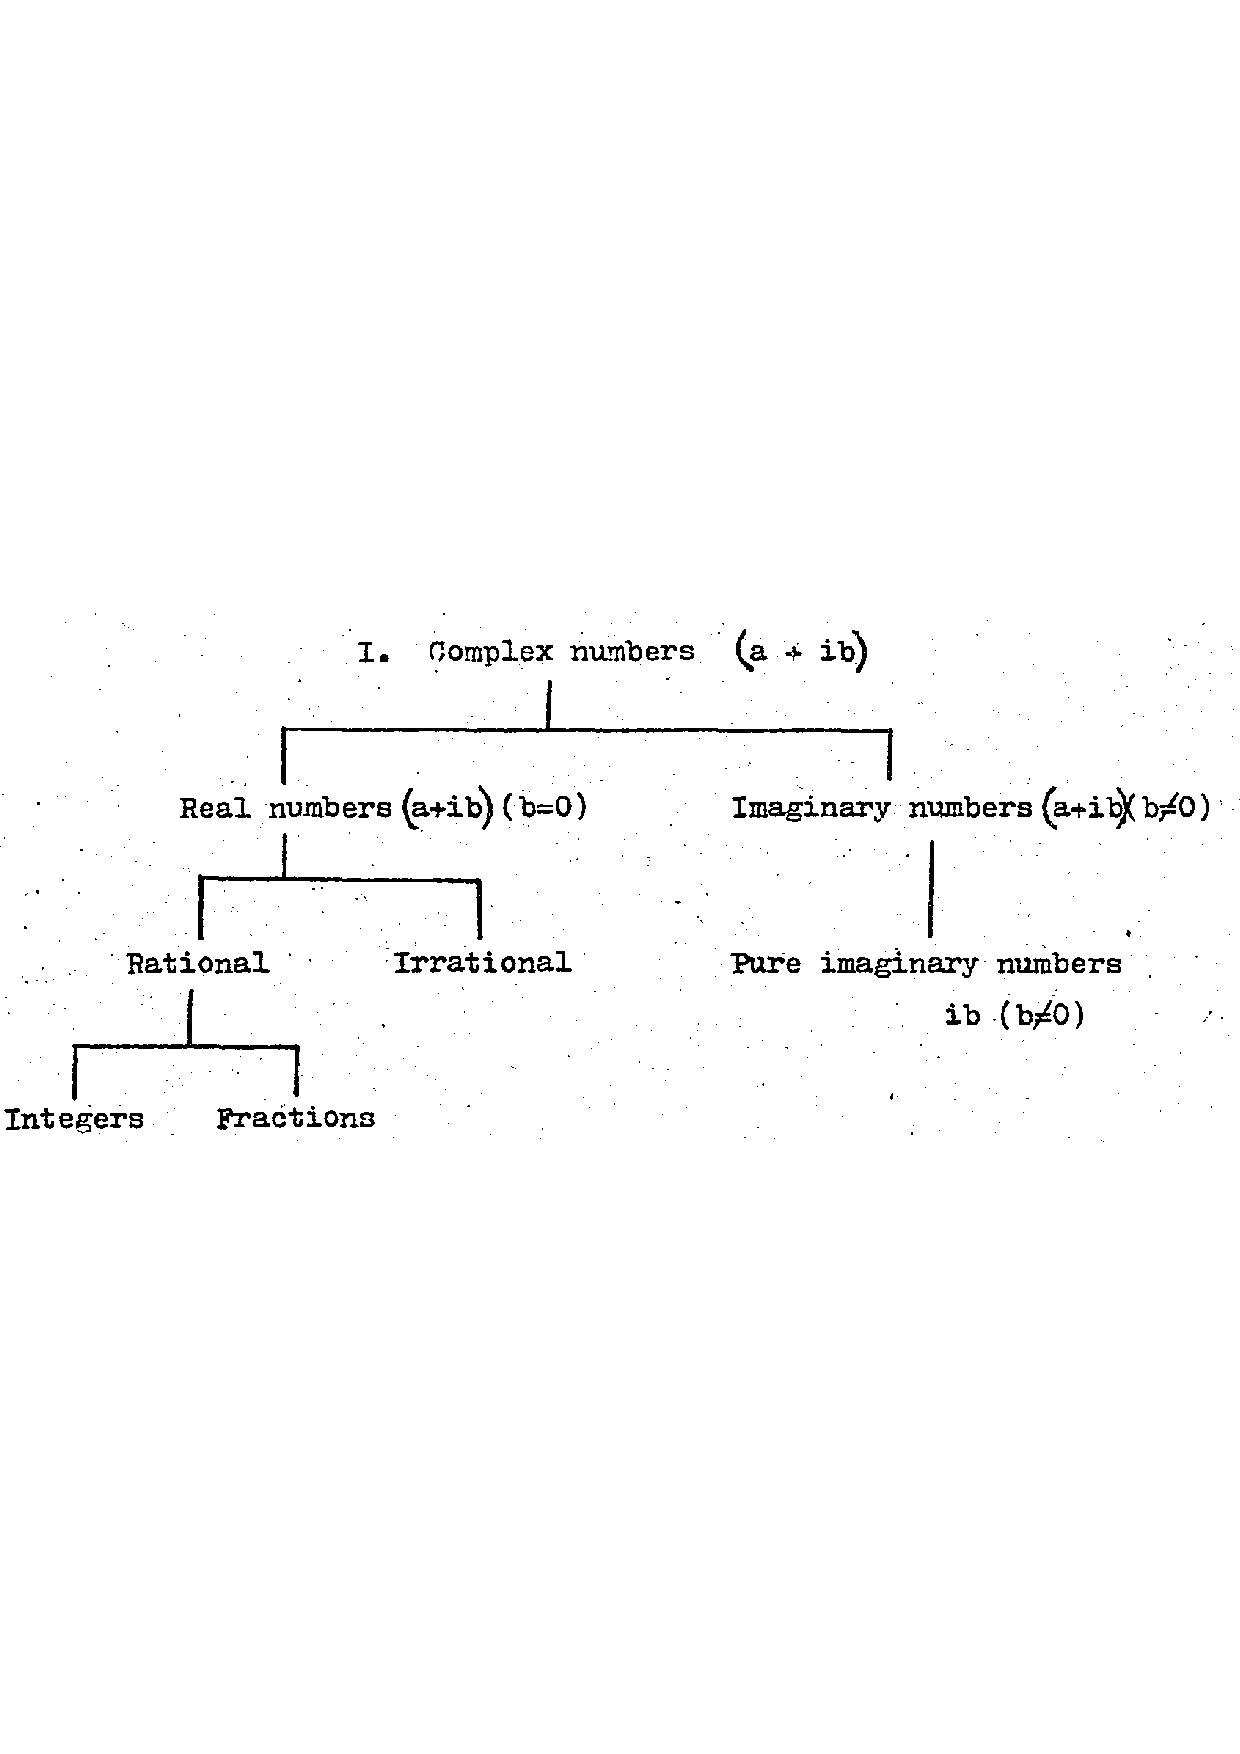
\includegraphics[width=0.9\textwidth]{images/SD-1-1p15A}
%	\caption{Classification of complex numbers}
%	\label{fig:classificationOfComplexNumbersA}
%\end{figure}

%\begin{center}
%\begin{tabular}{cc}
%\end{tabular}
%\end{center}

%\begin{exmp}
%\begin{hSolution}
%\end{hSolution}
%\end{exmp}

%\begin{hEnumerateAlpha}
%\end{hEnumerateAlpha}

%\begin{hEnumerateRoman}
%\end{hEnumerateRoman}

%$
%\begin{bmatrix}
%\end{bmatrix}
%$

%\frac{aaaa}{bbb}
%\frac{a_{n}}{b_{n}}
%\left( aaaa \right)
%\Longrightarrow

%\begin{multicols}{2}
%	bb
%\columnbreak
%	aa
%\end{multicols}
